\Transcb{yellow}{blue}{Het zichtbare heelal}
\twocolumn
\begin{center}
{\blue Electromagnetische straling}\\[5mm]

\includegraphics[keepaspectratio,width=5cm]{optical2}
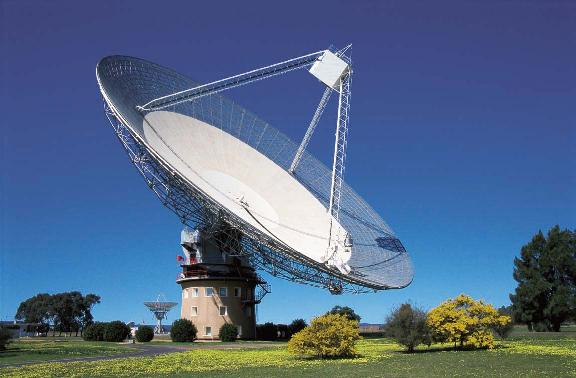
\includegraphics[keepaspectratio,width=7cm]{radio2}\\[1.5cm]
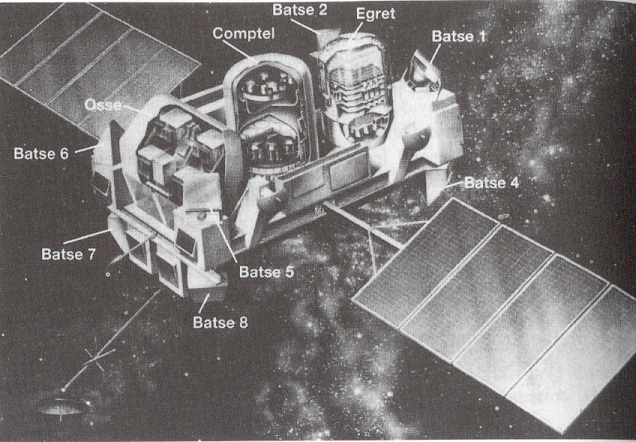
\includegraphics[keepaspectratio,width=12cm]{cgro}
\end{center}

\newpage

\vspace*{1mm}
\begin{center}
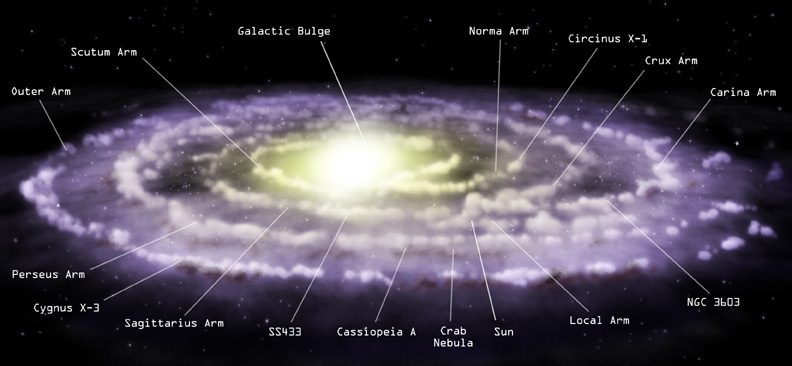
\includegraphics[keepaspectratio,width=13cm]{milky-way}\\[3mm]
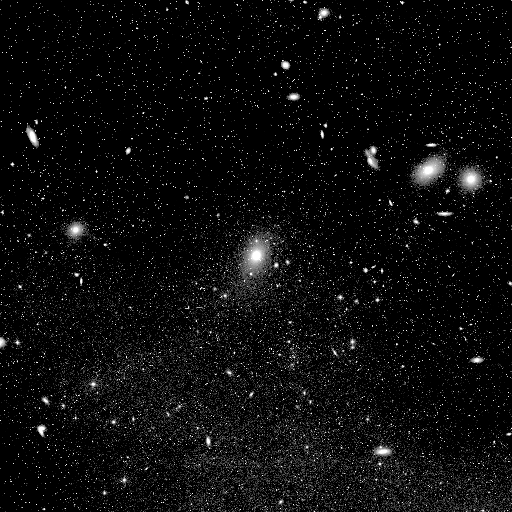
\includegraphics[keepaspectratio,height=8cm]{virgo}
\end{center}

\Tr
\vspace*{1mm}
\begin{itemize}
\item \colorbox{yellow}{Waar komt deze materie vandaan ?}
\end{itemize}
%
\vspace*{1cm}
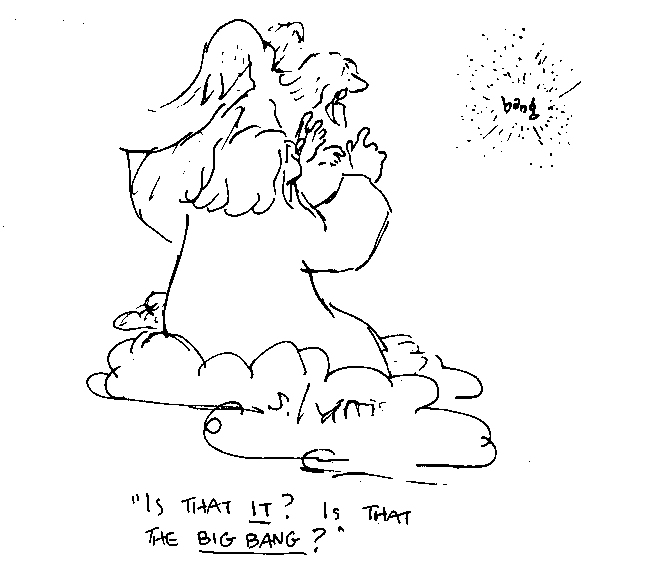
\includegraphics[keepaspectratio,width=12cm]{bang}

\newpage

\begin{itemize}
\item \colorbox{yellow}{Waarom zo "klonterig" verdeeld ?}
\item[] Onderlinge interacties
\item[]\begin{center}{\blue Mechanica (zwaartekracht)}\end{center}
\item \colorbox{yellow}{Wat laat de sterren stralen ?}
\item[] Nucleaire processen
\item[]\begin{center}{\blue Deeltjes fysica}\end{center}
\item \colorbox{yellow}{Emissie en absorbtie lijnen ?}
\item[] Atoom structuur
\item[]\begin{center}{\blue Quantum fysica}\end{center}
\item \colorbox{yellow}{Observatie verschoven spectraallijnen}
\item[] Uitdijend Heelal
\item[]\begin{center}{\blue Kosmologisch model}\end{center}
\end{itemize}
